\documentclass[ignorenonframetext,]{beamer}
\setbeamertemplate{caption}[numbered]
\setbeamertemplate{caption label separator}{: }
\setbeamercolor{caption name}{fg=normal text.fg}
\beamertemplatenavigationsymbolsempty
\usepackage{lmodern}
\usepackage{amssymb,amsmath}
\usepackage{ifxetex,ifluatex}
\usepackage{fixltx2e} % provides \textsubscript
\ifnum 0\ifxetex 1\fi\ifluatex 1\fi=0 % if pdftex
  \usepackage[T1]{fontenc}
  \usepackage[utf8]{inputenc}
\else % if luatex or xelatex
  \ifxetex
    \usepackage{mathspec}
  \else
    \usepackage{fontspec}
  \fi
  \defaultfontfeatures{Ligatures=TeX,Scale=MatchLowercase}
\fi
% use upquote if available, for straight quotes in verbatim environments
\IfFileExists{upquote.sty}{\usepackage{upquote}}{}
% use microtype if available
\IfFileExists{microtype.sty}{%
\usepackage{microtype}
\UseMicrotypeSet[protrusion]{basicmath} % disable protrusion for tt fonts
}{}
\newif\ifbibliography
\hypersetup{
            pdftitle={Decline in South Sound's Cancer magister Fishery},
            pdfauthor={Claudia Mateo},
            pdfborder={0 0 0},
            breaklinks=true}
\urlstyle{same}  % don't use monospace font for urls
\usepackage{color}
\usepackage{fancyvrb}
\newcommand{\VerbBar}{|}
\newcommand{\VERB}{\Verb[commandchars=\\\{\}]}
\DefineVerbatimEnvironment{Highlighting}{Verbatim}{commandchars=\\\{\}}
% Add ',fontsize=\small' for more characters per line
\usepackage{framed}
\definecolor{shadecolor}{RGB}{248,248,248}
\newenvironment{Shaded}{\begin{snugshade}}{\end{snugshade}}
\newcommand{\KeywordTok}[1]{\textcolor[rgb]{0.13,0.29,0.53}{\textbf{#1}}}
\newcommand{\DataTypeTok}[1]{\textcolor[rgb]{0.13,0.29,0.53}{#1}}
\newcommand{\DecValTok}[1]{\textcolor[rgb]{0.00,0.00,0.81}{#1}}
\newcommand{\BaseNTok}[1]{\textcolor[rgb]{0.00,0.00,0.81}{#1}}
\newcommand{\FloatTok}[1]{\textcolor[rgb]{0.00,0.00,0.81}{#1}}
\newcommand{\ConstantTok}[1]{\textcolor[rgb]{0.00,0.00,0.00}{#1}}
\newcommand{\CharTok}[1]{\textcolor[rgb]{0.31,0.60,0.02}{#1}}
\newcommand{\SpecialCharTok}[1]{\textcolor[rgb]{0.00,0.00,0.00}{#1}}
\newcommand{\StringTok}[1]{\textcolor[rgb]{0.31,0.60,0.02}{#1}}
\newcommand{\VerbatimStringTok}[1]{\textcolor[rgb]{0.31,0.60,0.02}{#1}}
\newcommand{\SpecialStringTok}[1]{\textcolor[rgb]{0.31,0.60,0.02}{#1}}
\newcommand{\ImportTok}[1]{#1}
\newcommand{\CommentTok}[1]{\textcolor[rgb]{0.56,0.35,0.01}{\textit{#1}}}
\newcommand{\DocumentationTok}[1]{\textcolor[rgb]{0.56,0.35,0.01}{\textbf{\textit{#1}}}}
\newcommand{\AnnotationTok}[1]{\textcolor[rgb]{0.56,0.35,0.01}{\textbf{\textit{#1}}}}
\newcommand{\CommentVarTok}[1]{\textcolor[rgb]{0.56,0.35,0.01}{\textbf{\textit{#1}}}}
\newcommand{\OtherTok}[1]{\textcolor[rgb]{0.56,0.35,0.01}{#1}}
\newcommand{\FunctionTok}[1]{\textcolor[rgb]{0.00,0.00,0.00}{#1}}
\newcommand{\VariableTok}[1]{\textcolor[rgb]{0.00,0.00,0.00}{#1}}
\newcommand{\ControlFlowTok}[1]{\textcolor[rgb]{0.13,0.29,0.53}{\textbf{#1}}}
\newcommand{\OperatorTok}[1]{\textcolor[rgb]{0.81,0.36,0.00}{\textbf{#1}}}
\newcommand{\BuiltInTok}[1]{#1}
\newcommand{\ExtensionTok}[1]{#1}
\newcommand{\PreprocessorTok}[1]{\textcolor[rgb]{0.56,0.35,0.01}{\textit{#1}}}
\newcommand{\AttributeTok}[1]{\textcolor[rgb]{0.77,0.63,0.00}{#1}}
\newcommand{\RegionMarkerTok}[1]{#1}
\newcommand{\InformationTok}[1]{\textcolor[rgb]{0.56,0.35,0.01}{\textbf{\textit{#1}}}}
\newcommand{\WarningTok}[1]{\textcolor[rgb]{0.56,0.35,0.01}{\textbf{\textit{#1}}}}
\newcommand{\AlertTok}[1]{\textcolor[rgb]{0.94,0.16,0.16}{#1}}
\newcommand{\ErrorTok}[1]{\textcolor[rgb]{0.64,0.00,0.00}{\textbf{#1}}}
\newcommand{\NormalTok}[1]{#1}
\usepackage{longtable,booktabs}
\usepackage{caption}
% These lines are needed to make table captions work with longtable:
\makeatletter
\def\fnum@table{\tablename~\thetable}
\makeatother
\usepackage{graphicx,grffile}
\makeatletter
\def\maxwidth{\ifdim\Gin@nat@width>\linewidth\linewidth\else\Gin@nat@width\fi}
\def\maxheight{\ifdim\Gin@nat@height>\textheight0.8\textheight\else\Gin@nat@height\fi}
\makeatother
% Scale images if necessary, so that they will not overflow the page
% margins by default, and it is still possible to overwrite the defaults
% using explicit options in \includegraphics[width, height, ...]{}
\setkeys{Gin}{width=\maxwidth,height=\maxheight,keepaspectratio}

% Prevent slide breaks in the middle of a paragraph:
\widowpenalties 1 10000
\raggedbottom

\AtBeginPart{
  \let\insertpartnumber\relax
  \let\partname\relax
  \frame{\partpage}
}
\AtBeginSection{
  \ifbibliography
  \else
    \let\insertsectionnumber\relax
    \let\sectionname\relax
    \frame{\sectionpage}
  \fi
}
\AtBeginSubsection{
  \let\insertsubsectionnumber\relax
  \let\subsectionname\relax
  \frame{\subsectionpage}
}

\setlength{\parindent}{0pt}
\setlength{\parskip}{6pt plus 2pt minus 1pt}
\setlength{\emergencystretch}{3em}  % prevent overfull lines
\providecommand{\tightlist}{%
  \setlength{\itemsep}{0pt}\setlength{\parskip}{0pt}}
\setcounter{secnumdepth}{0}

\title{Decline in South Sound's \emph{Cancer magister} Fishery}
\author{Claudia Mateo}
\date{11/21/2019}

\begin{document}
\frame{\titlepage}

\begin{frame}{Data}

\begin{itemize}
\tightlist
\item
  Catch data in lbs. was collated for marine areas 10, 11, and 13 from
  Washington Department of Fish and Wildlife catch records.
\item
  Combined, areas 10, 11, and 13 represent the Sound.
\item
  Areas 11 and 13 represent the South Sound.
\end{itemize}

\emph{Note concerning raw data}

\begin{itemize}
\tightlist
\item
  In all raw data, ending numerals in variable name represent marine
  area.
\end{itemize}

\end{frame}

\begin{frame}[fragile]{Marine areas 11 \& 13 catch data}

\begin{Shaded}
\begin{Highlighting}[]
\NormalTok{DC_catch.}\DecValTok{10}\NormalTok{ <-}\StringTok{ }\KeywordTok{read.csv}\NormalTok{(}\StringTok{"../Data/2007.2017_DC_catch.10.csv"}\NormalTok{, }\DataTypeTok{header =} \OtherTok{TRUE}\NormalTok{)}
\end{Highlighting}
\end{Shaded}

\begin{longtable}[]{@{}rr@{}}
\toprule
year & lbs\_dungeness.10\tabularnewline
\midrule
\endhead
2007 & 61429\tabularnewline
2008 & 50941\tabularnewline
2009 & 72231\tabularnewline
2010 & 119099\tabularnewline
2011 & 146080\tabularnewline
2012 & 168269\tabularnewline
2013 & 166382\tabularnewline
2014 & 202051\tabularnewline
2015 & 227500\tabularnewline
2016 & 150043\tabularnewline
2017 & 45603\tabularnewline
\bottomrule
\end{longtable}

\end{frame}

\begin{frame}[fragile]{Marina area 10 catch data}

\begin{Shaded}
\begin{Highlighting}[]
\NormalTok{DC_catch.}\FloatTok{11.13}\NormalTok{ <-}\StringTok{ }\KeywordTok{read.csv}\NormalTok{(}\StringTok{"../Data/2007.2017_DC_catch.csv"}\NormalTok{, }\DataTypeTok{header =} \OtherTok{TRUE}\NormalTok{)}
\end{Highlighting}
\end{Shaded}

\begin{longtable}[]{@{}rrr@{}}
\toprule
year & lbs\_dungeness.11 & lbs\_dungeness.13\tabularnewline
\midrule
\endhead
2007 & 44884 & 16822\tabularnewline
2008 & 43887 & 49906\tabularnewline
2009 & 62661 & 55714\tabularnewline
2010 & 86842 & 118734\tabularnewline
2011 & 107368 & 69200\tabularnewline
2012 & 89262 & 65899\tabularnewline
2013 & 88295 & 49983\tabularnewline
2014 & 106686 & 37262\tabularnewline
2015 & 87185 & 24856\tabularnewline
2016 & 24524 & 8350\tabularnewline
2017 & 16341 & 4226\tabularnewline
\bottomrule
\end{longtable}

\end{frame}

\begin{frame}[fragile]{Stitching tables}

\begin{Shaded}
\begin{Highlighting}[]
\NormalTok{DC_catch <-}\StringTok{ }\KeywordTok{inner_join}\NormalTok{(DC_catch.}\DecValTok{10}\NormalTok{, DC_catch.}\FloatTok{11.13}\NormalTok{, }\DataTypeTok{by =} \StringTok{"year"}\NormalTok{)}
\end{Highlighting}
\end{Shaded}

There is now a single table describing the catch rates in lbs. at marine
areas 10, 11, and 13.

\begin{Shaded}
\begin{Highlighting}[]
\KeywordTok{head}\NormalTok{(DC_catch)}
\end{Highlighting}
\end{Shaded}

\begin{verbatim}
##   year lbs_dungeness.10 lbs_dungeness.11 lbs_dungeness.13
## 1 2007            61429            44884            16822
## 2 2008            50941            43887            49906
## 3 2009            72231            62661            55714
## 4 2010           119099            86842           118734
## 5 2011           146080           107368            69200
## 6 2012           168269            89262            65899
\end{verbatim}

\end{frame}

\begin{frame}[fragile]{Editing column names}

The column names need to be changed to making data tidying simpler.

\begin{Shaded}
\begin{Highlighting}[]
\NormalTok{DC_catch_renamed <-}\StringTok{ }\NormalTok{DC_catch }\OperatorTok\StringTok{ }\KeywordTok{rename}\NormalTok{(}\StringTok{"10"}\NormalTok{ =}\StringTok{ }\NormalTok{lbs_dungeness.}\DecValTok{10}\NormalTok{, }
                                     \StringTok{"11"}\NormalTok{ =}\StringTok{ }\NormalTok{lbs_dungeness.}\DecValTok{11}\NormalTok{, }\StringTok{"13"}\NormalTok{ =}\StringTok{ }\NormalTok{lbs_dungeness.}\DecValTok{13}\NormalTok{)}
\KeywordTok{head}\NormalTok{(DC_catch_renamed)}
\end{Highlighting}
\end{Shaded}

\begin{verbatim}
##   year     10     11     13
## 1 2007  61429  44884  16822
## 2 2008  50941  43887  49906
## 3 2009  72231  62661  55714
## 4 2010 119099  86842 118734
## 5 2011 146080 107368  69200
## 6 2012 168269  89262  65899
\end{verbatim}

\end{frame}

\begin{frame}[fragile]{Gathering data}

The tidyr gather function can be used to separate the lbs observation
columns into two columns; one column describing the area and one the
number of lbs.

\begin{Shaded}
\begin{Highlighting}[]
\NormalTok{DC_catch_tidy <-}\StringTok{ }\NormalTok{DC_catch_renamed }\OperatorTok\StringTok{ }
\StringTok{  }\KeywordTok{gather}\NormalTok{(}\StringTok{`}\DataTypeTok{10}\StringTok{`}\NormalTok{, }\StringTok{`}\DataTypeTok{11}\StringTok{`}\NormalTok{, }\StringTok{`}\DataTypeTok{13}\StringTok{`}\NormalTok{, }\DataTypeTok{key =} \StringTok{"area"}\NormalTok{, }\DataTypeTok{value =} \StringTok{"lbs"}\NormalTok{)}
\KeywordTok{head}\NormalTok{(DC_catch_tidy)}
\end{Highlighting}
\end{Shaded}

\begin{verbatim}
##   year area    lbs
## 1 2007   10  61429
## 2 2008   10  50941
## 3 2009   10  72231
## 4 2010   10 119099
## 5 2011   10 146080
## 6 2012   10 168269
\end{verbatim}

\end{frame}

\begin{frame}{Plot of main data}

Shows the growth and decline of the \emph{C. magister} fishery in marine
areas 10, 11, and 13 through pounds caught between 2007 and 2017.

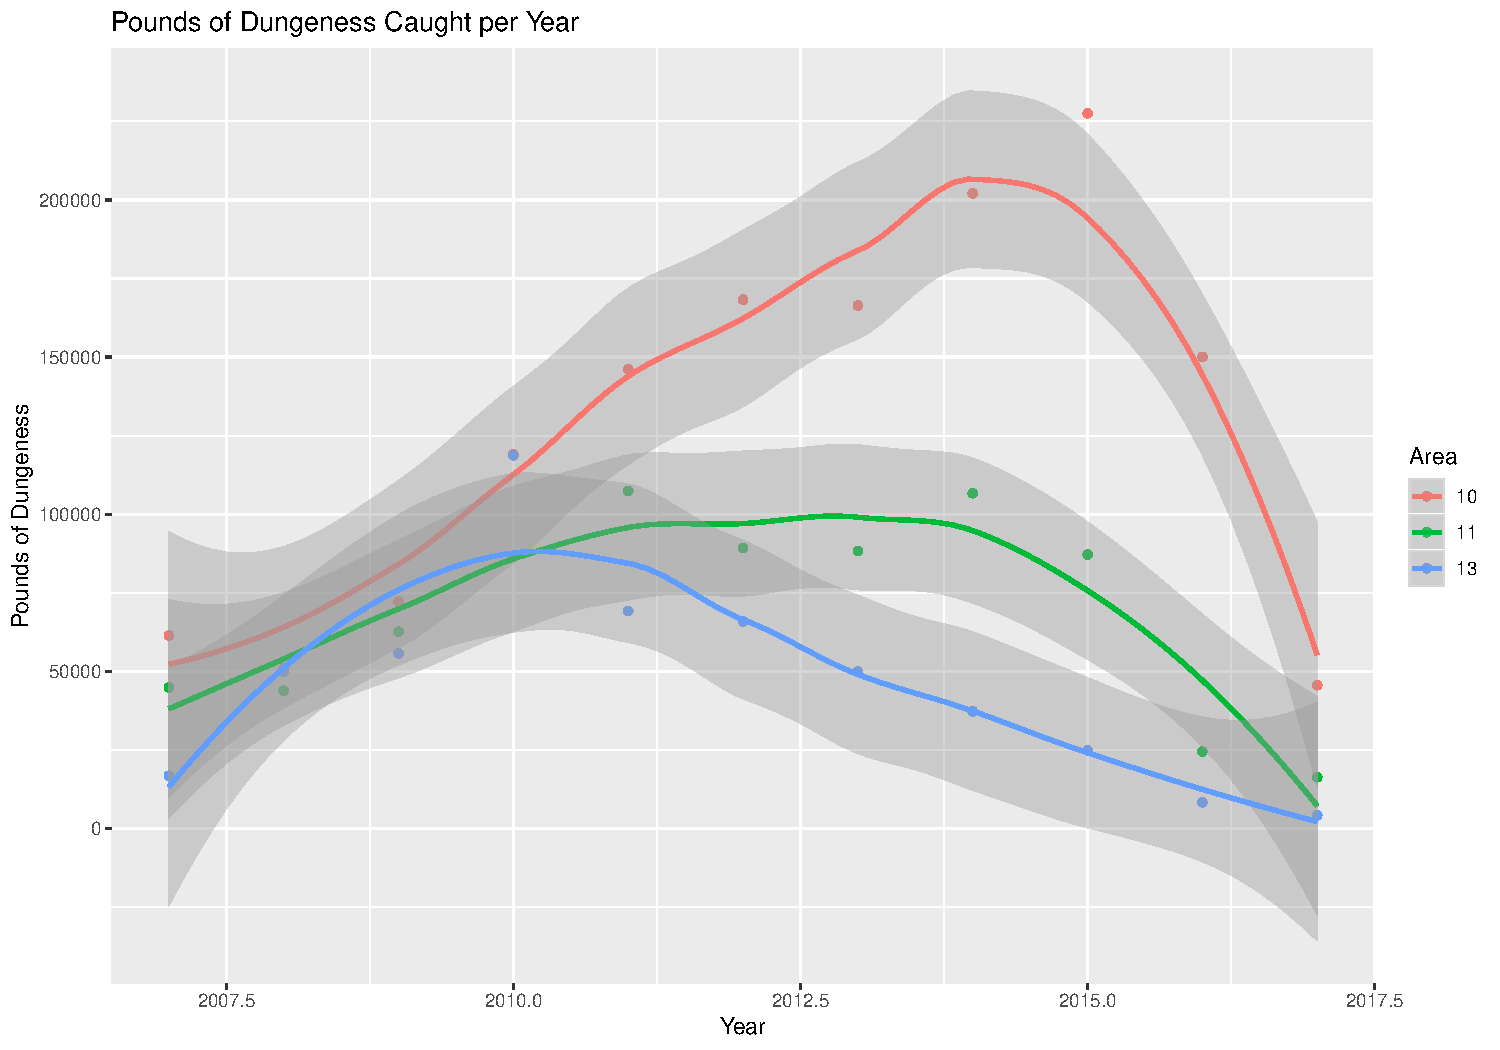
\includegraphics{Claudia-dungeness_files/figure-beamer/main plot-1.pdf}

This graph uses the DC\_catch\_tidy dataframe.

\end{frame}

\begin{frame}[fragile]{Analysis}

Looking for trends within the main plot.

\textbf{Data subsets for analysis}

\begin{Shaded}
\begin{Highlighting}[]
\NormalTok{lin_data.}\DecValTok{10}\NormalTok{ <-}\StringTok{ }\KeywordTok{subset}\NormalTok{(DC_catch, year }\OperatorTok\StringTok{ }\KeywordTok{c}\NormalTok{(}\StringTok{"2013"}\NormalTok{, }\StringTok{"2014"}\NormalTok{, }\StringTok{"2015"}\NormalTok{, }\StringTok{"2016"}\NormalTok{, }\StringTok{"2017"}\NormalTok{))}
\NormalTok{lin_data.}\DecValTok{11}\NormalTok{ <-}\StringTok{ }\KeywordTok{subset}\NormalTok{(DC_catch, year }\OperatorTok\StringTok{ }\KeywordTok{c}\NormalTok{(}\StringTok{"2014"}\NormalTok{, }\StringTok{"2015"}\NormalTok{, }\StringTok{"2016"}\NormalTok{, }\StringTok{"2017"}\NormalTok{))}
\NormalTok{lin_data.}\DecValTok{13}\NormalTok{ <-}\StringTok{ }\KeywordTok{subset}\NormalTok{(DC_catch, year }\OperatorTok\StringTok{ }\KeywordTok{c}\NormalTok{(}\StringTok{"2011"}\NormalTok{, }\StringTok{"2012"}\NormalTok{, }\StringTok{"2013"}\NormalTok{, }\StringTok{"2014"}\NormalTok{, }
                                            \StringTok{"2015"}\NormalTok{, }\StringTok{"2016"}\NormalTok{, }\StringTok{"2017"}\NormalTok{))}
\end{Highlighting}
\end{Shaded}

Subsets focus in on a particular part of the data showing a decline.

\end{frame}

\begin{frame}{Linear models using subsets}

\begin{figure}
\centering
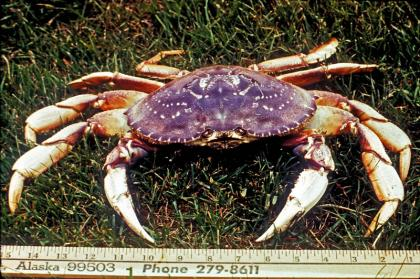
\includegraphics{../Images/dungeness_crab.jpg}
\caption{\emph{C. magister}}
\end{figure}

All linear models are created using the DC\_catch dataframe.

\end{frame}

\begin{frame}[fragile]{Liner model - Area 10}

\begin{Shaded}
\begin{Highlighting}[]
\KeywordTok{summary}\NormalTok{(lm_fit.}\DecValTok{10}\NormalTok{)}
\end{Highlighting}
\end{Shaded}

\begin{verbatim}
## 
## Call:
## lm(formula = year ~ lbs_dungeness.10, data = lin_data.10)
## 
## Residuals:
##       7       8       9      10      11 
## -1.8788 -0.3428  1.0396  0.8757  0.3064 
## 
## Coefficients:
##                    Estimate Std. Error  t value Pr(>|t|)    
## (Intercept)       2.017e+03  1.662e+00 1213.759 1.23e-09 ***
## lbs_dungeness.10 -1.503e-05  9.765e-06   -1.539    0.221    
## ---
## Signif. codes:  0 '***' 0.001 '**' 0.01 '*' 0.05 '.' 0.1 ' ' 1
## 
## Residual standard error: 1.365 on 3 degrees of freedom
## Multiple R-squared:  0.4411, Adjusted R-squared:  0.2548 
## F-statistic: 2.368 on 1 and 3 DF,  p-value: 0.2215
\end{verbatim}

\end{frame}

\begin{frame}[fragile]{Linear model - Area 11}

\begin{Shaded}
\begin{Highlighting}[]
\KeywordTok{summary}\NormalTok{(lm_fit.}\DecValTok{11}\NormalTok{)}
\end{Highlighting}
\end{Shaded}

\begin{verbatim}
## 
## Call:
## lm(formula = year ~ lbs_dungeness.11, data = lin_data.11)
## 
## Residuals:
##       8       9      10      11 
## -0.1819  0.2826 -0.4380  0.3373 
## 
## Coefficients:
##                    Estimate Std. Error  t value Pr(>|t|)    
## (Intercept)       2.017e+03  4.134e-01 4878.769  4.2e-08 ***
## lbs_dungeness.11 -2.746e-05  5.869e-06   -4.679   0.0428 *  
## ---
## Signif. codes:  0 '***' 0.001 '**' 0.01 '*' 0.05 '.' 0.1 ' ' 1
## 
## Residual standard error: 0.4575 on 2 degrees of freedom
## Multiple R-squared:  0.9163, Adjusted R-squared:  0.8744 
## F-statistic: 21.89 on 1 and 2 DF,  p-value: 0.04277
\end{verbatim}

\end{frame}

\begin{frame}[fragile]{Linear model - Area 13}

\begin{Shaded}
\begin{Highlighting}[]
\KeywordTok{summary}\NormalTok{(lm_fit.}\DecValTok{13}\NormalTok{)}
\end{Highlighting}
\end{Shaded}

\begin{verbatim}
## 
## Call:
## lm(formula = year ~ lbs_dungeness.13, data = lin_data.13)
## 
## Residuals:
##        5        6        7        8        9       10       11 
## -0.36599  0.36305  0.05660  0.01241 -0.00593 -0.36081  0.30067 
## 
## Coefficients:
##                    Estimate Std. Error t value Pr(>|t|)    
## (Intercept)       2.017e+03  2.169e-01 9300.90  < 2e-16 ***
## lbs_dungeness.13 -8.208e-05  4.898e-06  -16.76 1.38e-05 ***
## ---
## Signif. codes:  0 '***' 0.001 '**' 0.01 '*' 0.05 '.' 0.1 ' ' 1
## 
## Residual standard error: 0.313 on 5 degrees of freedom
## Multiple R-squared:  0.9825, Adjusted R-squared:  0.979 
## F-statistic: 280.9 on 1 and 5 DF,  p-value: 1.382e-05
\end{verbatim}

\textbf{Analysis findings} There is no significant decrease in catch
rate in marine area 10, however there is a significant decrease in areas
11 and 13.

\end{frame}

\begin{frame}{Subset plots}

Shows a significant decrease in \emph{C. magister} catch from 2014 to
2017.

\begin{figure}
\centering
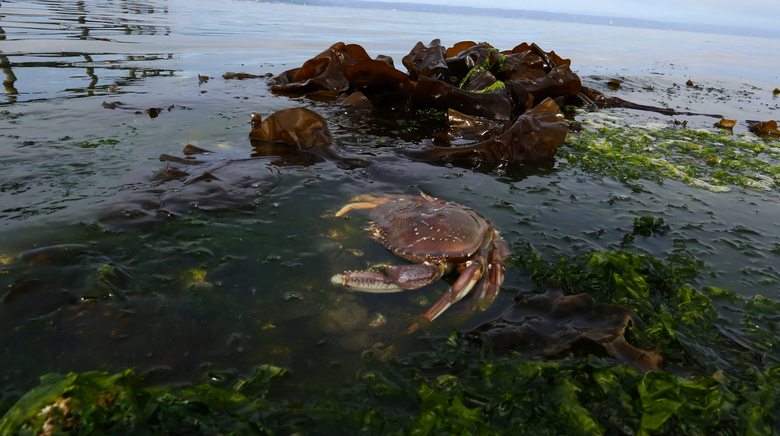
\includegraphics{../Images/dungeness_decline.jpg}
\caption{\emph{C. magister} in a poor habitat}
\end{figure}

\end{frame}

\begin{frame}{Marine area 11}

This graph shows a significant decrease in \emph{C. magister} catch from
2014 to 2017.

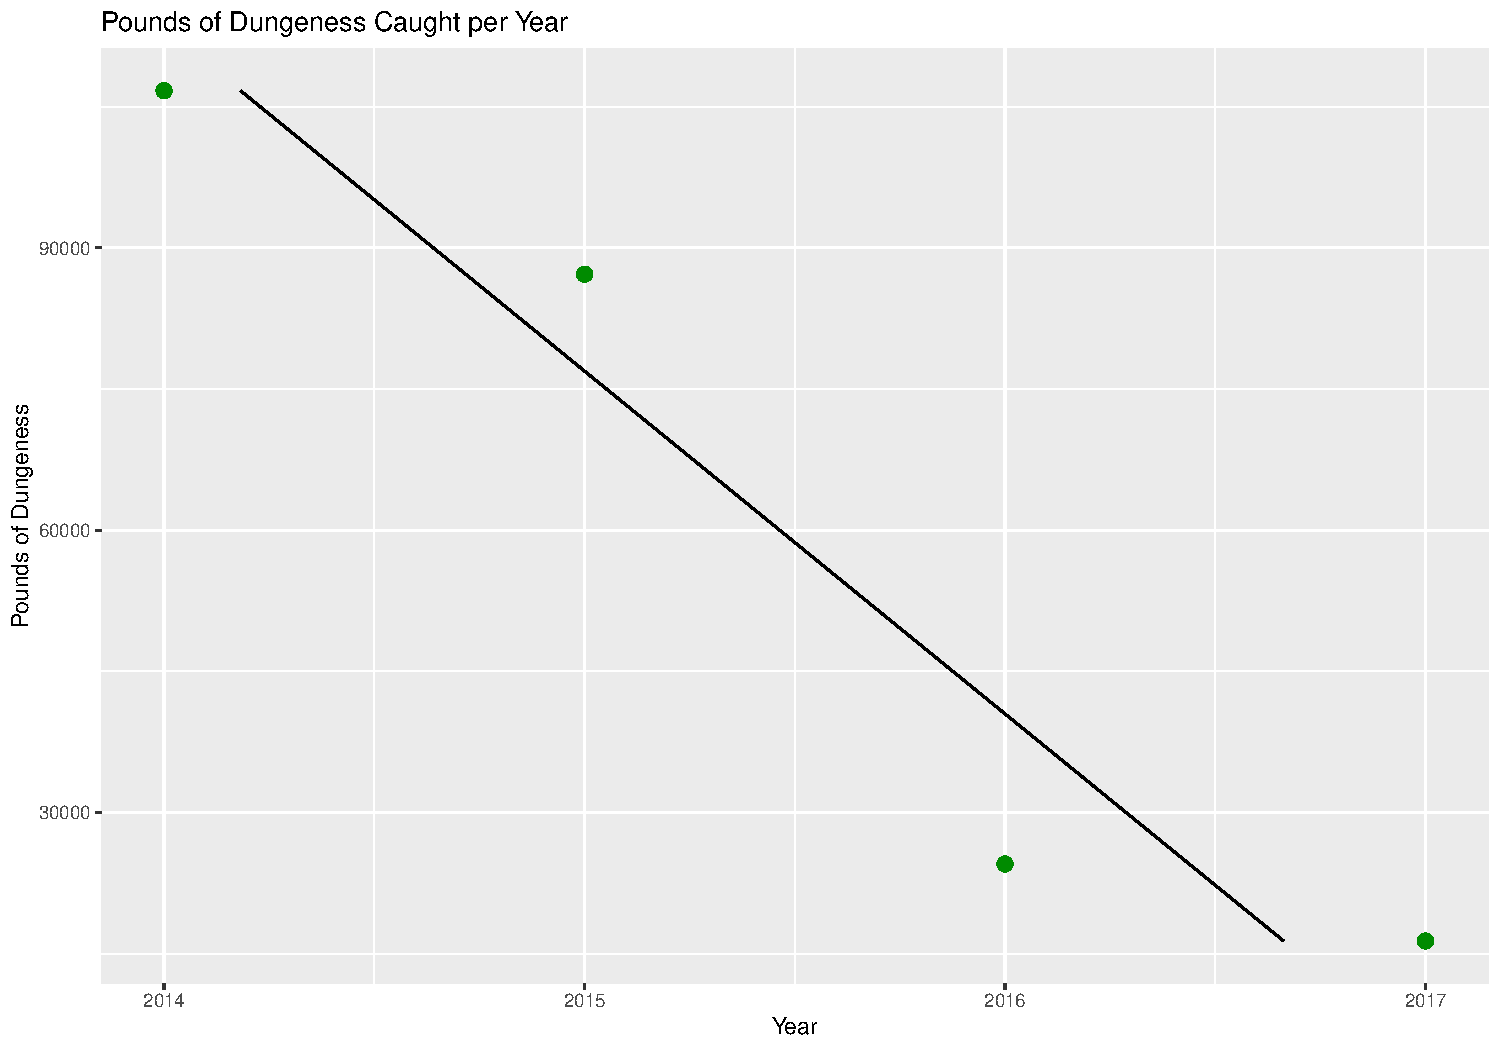
\includegraphics{Claudia-dungeness_files/figure-beamer/subset plot area 11-1.pdf}

\end{frame}

\begin{frame}{Marine area 13}

This graph shows a significant decrease in \emph{C. magister} catch from
2011 to 2017.

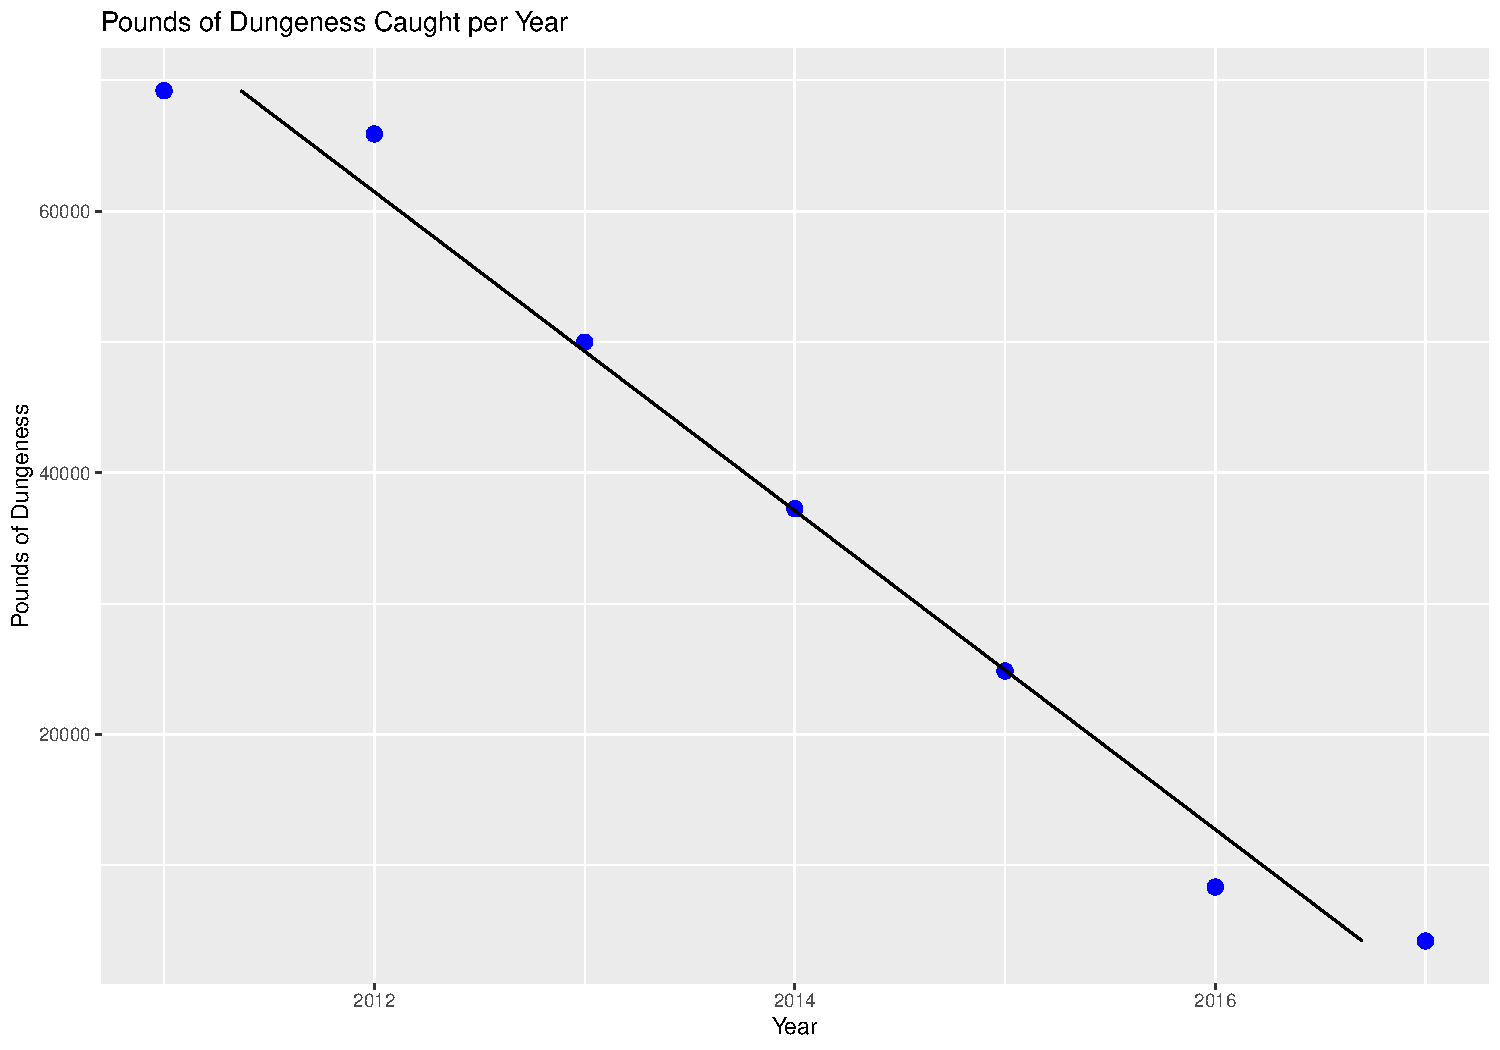
\includegraphics{Claudia-dungeness_files/figure-beamer/subset plot area 13-1.pdf}

\end{frame}

\end{document}
